\chapter{Antiferromagnetism in the HM}\label{app:hm-af-ground-state}

In this appendix we give some details about the antiferromagnetic phase in the conventional Hubbard model,
\begin{equation}\label{appeq:hm}
	\hat H = 
	-t \sum_{\langle ij \rangle} \sum_\sigma \left[
	\hat c_{i\sigma}^\dagger \hat c_{j\sigma} + \hc
	\right]
	+ U \sum_i \hat n_{i\uparrow} \hat n_{i\downarrow}
	\qquad
	t, U  > 0
\end{equation}
approximated by HF methods. We use the results discussed in Sec.~\ref{subsec:af-hm}. 

Let the Nambu spinors:
\[
	\hat \Psi_{\mathbf{k}\sigma} \equiv \begin{bmatrix}
		\hat c_{\mathbf{k}\sigma} \\
		\hat c_{\mathbf{k}+\bm{\pi}\sigma} 
	\end{bmatrix}
\]
Let also the gap function:
\[
	\Delta_{\mathbf{k}\sigma} = (-1)^{\delta_{\sigma=\downarrow}} mU
\]
We know from Eq.~\eqref{eq:af-hm-spin-h} that the approximated hamiltonian is:
\[
	\hat H_t + \hat H_U \simeq \sum_{\mathbf{k} \in \mathrm{MBZ}} \sum_\sigma \mathbf{b}_{\mathbf{k}\sigma} \cdot \hat{\mathbf{s}}_{\mathbf{k}\sigma} + nU \hat N - E_{\mathrm{H}/U}^{(\mathrm{AF})}
\]
where:
\[
	\mathbf{b}_{\mathbf{k}\sigma} \equiv \begin{bmatrix}
		-\Delta_{\mathbf{k}\sigma} \\ 0 \\ \epsilon_{\mathbf{k}\sigma} 
	\end{bmatrix} 
	\qquad
	\hat s_{\mathbf{k}\sigma}^\alpha \equiv \hat \Psi_{\mathbf{k}\sigma}^\dagger \tau^\alpha \hat \Psi_{\mathbf{k}\sigma}
	\qquad
	\hat{\mathbf{s}}_{\mathbf{k}\sigma} \equiv \begin{bmatrix}
		\hat s_{\mathbf{k}\sigma}^x \\
		\hat s_{\mathbf{k}\sigma}^y \\
		\hat s_{\mathbf{k}\sigma}^z
	\end{bmatrix}
\]
Through the unitary matrix $W_{\mathbf{k}\sigma}$ given in Eq.~\eqref{eq:af-hm-diagonalizer}, the hamiltonian is mapped to a gas of non-interacting fermions collected in the $\hat \Gamma$ spinors of Eq.~\eqref{eq:af-Gamma=WPsi},
\[
	\hat\Gamma_{\mathbf{k}\sigma} = W_{\mathbf{k}\sigma} \hat \Psi_{\mathbf{k}\sigma} = \begin{bmatrix}
		\hat \gamma_{\mathbf{k}\sigma}^{(+)} \\ \hat \gamma_{\mathbf{k}\sigma}^{(-)}
	\end{bmatrix}
\]
The final non-interacting hamiltonian is:
\[
	\hat H_t + \hat H_U \simeq \sum_{\mathbf{k} \in \mathrm{MBZ}} \sum_\sigma E_{\mathbf{k}\sigma} \left(
		\hat \gamma_{\mathbf{k}\sigma}^{(+)\dagger} \hat \gamma_{\mathbf{k}\sigma}^{(+)} - \hat \gamma_{\mathbf{k}\sigma}^{(-)\dagger} \hat \gamma_{\mathbf{k}\sigma}^{(-)}
	\right) + nU \hat N -  E_{\mathrm{H}/U}^{(\mathrm{AF})}
\]
with $E_{\mathbf{k}\sigma}$ the Bogoliubov bands of Eq.~\eqref{eq:af-bands}. In next section we give the explicit form of the many-body ground-state at zero temperature and half-filling. From now on, limitedly to this appendix, we use the simplified notation:
\[
	\Delta_{\mathbf{k}\uparrow} \quad\to\quad \Delta
\]
with $\Delta_{\mathbf{k}\uparrow} = -\Delta_{\mathbf{k}\downarrow}$, and $\Delta=mU$.

\section{Explicit AF ground state at half-filling and $\beta \to \infty$}\label{appsubsec:af-T=0-gs}

Let $\ket{\Uparrow_{\mathbf{k}\sigma}}$ and $\ket{\Downarrow_{\mathbf{k}\sigma}}$ be respectively the ``up'' and ``down'' $\mathbf{k}$-th pseudo-spin states. Let $\ket{\overline{\Downarrow}_{\mathbf{k}\sigma}}$ be the ``down'' state in the tilted frame. The ground state is given by
\begin{equation}\label{appeq:af-hm-gs-1}
	\ket{\Psi} \equiv \bigotimes_\sigma \bigotimes_{\mathbf{k}\in\mathrm{MBZ}} \ket{\overline{\Downarrow}_{\mathbf{k}\sigma}}
\end{equation}
We can link the ``down'' states via an inverse rotation,
\begin{align}
	\ket{\overline{\Downarrow}_{\mathbf{k}\sigma}} &= e^{-i\theta_{\mathbf{k}\sigma} \hat s_{\mathbf{k}\sigma}^y} \ket{\Downarrow_{\mathbf{k}\sigma}} \nonumber \\
	&= \cos \theta_{\mathbf{k}\sigma} \ket{\Downarrow_{\mathbf{k}\sigma}} - i \sin\theta_{\mathbf{k}\sigma} \hat s_{\mathbf{k}\sigma}^y \ket{\Downarrow_{\mathbf{k}\sigma}} \nonumber \\
	&= \cos \theta_{\mathbf{k}\sigma} \ket{\Downarrow_{\mathbf{k}\sigma}} - \sin\theta_{\mathbf{k}\sigma} (\hat s_{\mathbf{k}\sigma}^+ - \hat s_{\mathbf{k}\sigma}^-) \ket{\Downarrow_{\mathbf{k}\sigma}} \nonumber \\
	&= \cos \theta_{\mathbf{k}\sigma} \ket{\Downarrow_{\mathbf{k}\sigma}} - \sin\theta_{\mathbf{k}\sigma} \ket{\Uparrow_{\mathbf{k}\sigma}} \label{appeq:af-hm-tilted-down}
\end{align}
having we used
\[
	\hat s_{\mathbf{k}\sigma}^\pm \equiv \frac{\hat s_{\mathbf{k}\sigma}^x \pm i\hat s_{\mathbf{k}\sigma}^y}{2}
\]

Use now Eqns.~\eqref{eq:af-hm-id-def} and \eqref{eq:af-hm-z-psi},
\[
	\frac{\hat \Id_{\mathbf{k}\sigma} + \hat s_{\mathbf{k}\sigma}^z}{2} = \hat n_{\mathbf{k}\sigma}
	\qquad
	\frac{\hat \Id_{\mathbf{k}\sigma} - \hat s_{\mathbf{k}\sigma}^z}{2} = \hat n_{\mathbf{k}+\bm{\pi}\sigma}
\]
Evaluating the above operators on the ``up'' and ``down'' states, we get
\[
\begin{aligned}
	\frac{1}{2} \mel{\Uparrow_{\mathbf{k}\sigma}}{\hat \Id_{\mathbf{k}\sigma} + \hat s_{\mathbf{k}\sigma}^z}{\Uparrow_{\mathbf{k}\sigma}} &= 1 \\
	\frac{1}{2} \mel{\Downarrow_{\mathbf{k}\sigma}}{\hat \Id_{\mathbf{k}\sigma} + \hat s_{\mathbf{k}\sigma}^z}{\Downarrow_{\mathbf{k}\sigma}} &= 0
\end{aligned}
\qquad
\begin{aligned}
	\frac{1}{2} \mel{\Uparrow_{\mathbf{k}\sigma}}{\hat \Id_{\mathbf{k}\sigma} - \hat s_{\mathbf{k}\sigma}^z}{\Uparrow_{\mathbf{k}\sigma}} &= 0 \\
	\frac{1}{2} \mel{\Downarrow_{\mathbf{k}\sigma}}{\hat \Id_{\mathbf{k}\sigma} - \hat s_{\mathbf{k}\sigma}^z}{\Downarrow_{\mathbf{k}\sigma}} &= 1
\end{aligned}
\]
Thus, up to a phase
\[
	\ket{\Uparrow_{\mathbf{k}\sigma}} \sim \hat c_{\mathbf{k}\sigma}^\dagger \ket{\Omega_{\mathbf{k}\sigma}}
	\qquad
	\ket{\Downarrow_{\mathbf{k}\sigma}} \sim \hat c_{\mathbf{k}+\bm{\pi}\sigma}^\dagger \ket{\Omega_{\mathbf{k}\sigma}}
\]
being $\ket{\Omega_{\mathbf{k}\sigma}}$ the $(\mathbf{k},\sigma)$ Hilbert subspace vacuum. 

It follows that composing Eqns.~\eqref{appeq:af-hm-gs-1} and \eqref{appeq:af-hm-tilted-down} the ground state $\ket{\Psi}$ can be written as:
\begin{equation}\label{appeq:af-hm-gs-2}
	\ket{\Psi} = \bigotimes_\sigma \bigotimes_{\mathbf{k}\in\mathrm{MBZ}} \left[
	\sin\theta_{\mathbf{k}\sigma} \hat c_{\mathbf{k}\sigma}^\dagger + e^{2i\zeta_{\mathbf{k}\sigma}} \cos \theta_{\mathbf{k}\sigma} \hat c_{\mathbf{k}+\bm{\pi}\sigma}^\dagger
	\right] \ket{\Omega_{\mathbf{k}\sigma}}
\end{equation}
having we absorbed in the relative phase $e^{2i\zeta_{\mathbf{k}\sigma}}$ the two states phases differences as well as the original sign difference of Eq.~\eqref{appeq:af-hm-tilted-down}. Now, inserting the explicit form of the ground state from equation above:
\[
\begin{aligned}
	\mel{\overline{\Downarrow}_{\mathbf{k}\sigma}}{\hat \psi_{\mathbf{k}\sigma} + \hat \psi_{\mathbf{k}\sigma}^\dagger}{\overline{\Downarrow}_{\mathbf{k}\sigma}} &= \left(e^{2i\zeta_{\mathbf{k}\sigma}} + e^{-2i\zeta_{\mathbf{k}\sigma}}\right) \sin\theta_{\mathbf{k}\sigma} \cos\theta_{\mathbf{k}\sigma} \\
	&= \cos 2\zeta_{\mathbf{k}\sigma} \sin 2\theta_{\mathbf{k}\sigma}
\end{aligned}
\]
but from Eq.~\eqref{eq:af-hm-x-psi}
\[
\begin{aligned}
	\mel{\overline{\Downarrow}_{\mathbf{k}\sigma}}{\hat \psi_{\mathbf{k}\sigma} + \hat \psi_{\mathbf{k}\sigma}^\dagger}{\overline{\Downarrow}_{\mathbf{k}\sigma}} &= 	\mel{\overline{\Downarrow}_{\mathbf{k}\sigma}}{\hat s_{\mathbf{k}\sigma}^x}{\overline{\Downarrow}_{\mathbf{k}\sigma}} \\
	&= \sin 2\theta_{\mathbf{k}\sigma}
\end{aligned}
\]
since the pseudofield has no $y$ component. This implies necessarily
\[
	\cos 2\zeta_{\mathbf{k}\sigma}
	\quad\implies\quad
	\zeta_{\mathbf{k}\sigma} = k\pi
	\qq{with}
	k\in\mathbb{Z}
\]
and lets us conclude from Eq.~\eqref{appeq:af-hm-gs-2}
\begin{equation}\label{appeq:af-hm-gs-3}
	\ket{\Psi} = \bigotimes_\sigma \bigotimes_{\mathbf{k}\in\mathrm{MBZ}} \left[
	\sin \theta_{\mathbf{k}\sigma} \hat c_{\mathbf{k}\sigma}^\dagger + \cos \theta_{\mathbf{k}\sigma} \hat c_{\mathbf{k}+\bm{\pi}\sigma}^\dagger
	\right] \ket{\Omega_{\mathbf{k}\sigma}}
\end{equation}
For low-temperature physics, we can expect the ground-state density matrix to be highly dominated by this BCS-like zero-temperature ground-state, which highlights the essential features of the system. 

Finally, using Eq.~\eqref{eq:af-Gamma=WPsi}, we check that correctly the ground-state describes a perfect degenerate $\gamma^{(-)}$ quasiparticles Fermi gas,
\begin{equation}\label{appeq:af-hm-gs-4}
	\ket{\Psi} = \bigotimes_\sigma \bigotimes_{\mathbf{k}\in\mathrm{MBZ}} \gamma_{\mathbf{k}\sigma}^{(-)\dagger} \ket{\Omega_{\mathbf{k}\sigma}}
\end{equation}
The AF phase can be thought of as a long-range coordination between fermionic states related by a $\bm{\pi}$ shift in reciprocal space, producing a new free gas where all interactions have been ``condensed'' in these AF pairs.

\section{Instability of the commensurate AF phase}\label{appsubsec:af-instability}

The commensurate AF phase is unstable at any finite doping. This result is discussed in \cite{singh1990collective,singh1991doped}, and here we recall just the main passages. Consider the local spin operator defined in Eq.~\eqref{eq:local-S},
\[
	\hat S_j^\alpha = \frac{1}{2} \hat \Psi_j^\dagger \tau^\alpha \hat \Psi_j
	\qquad
	\hat S_j^+ \equiv \frac{\hat S_j^x + i\hat S_j^y}{2}
	\qquad
	\hat S_j^- \equiv \frac{\hat S_j^x - i\hat S_j^y}{2}
\]
Let us take a continuum limit, $L_x \to \infty$ and $L_y \to \infty$, while the lattice spacing goes to zero.

Continuous SSBs are connected to the presence of a stable gapless Golstone mode. Such a Goldstone mode is essentially a sharp peak at zero frequency for some dressed response function. For the commensurate AF phase, the low-energy collective excitations are transverse spin fluctuations about the antiferromagnetic ground-state, describing SDWs. In order to see if the Golstone mode is stable for a given doping $\delta$, we need to investigate whether the respective response function diverges at zero frequency. If it does, we have a gapless Goldstone mode and the phase is stable; if not, the phase is unstable. We work at $\omega=0$ in order to capture gapless modes.

Consider the interaction representation of spin operators. Our new local spin operators are given by
\[
	\hat{\mathbf{S}}(\mathbf{r},t)
\]
The retarded transverse spin-spin response is given by:
\[
	\chi^{-+}(\mathbf{r},t;\mathbf{r}',t') =\equiv i \mathrm{H}(t-t') \mel{\Psi}{\comm{\hat S^-(\mathbf{r},t)}{\hat S^+(\mathbf{r}',t')}}{\Psi}
\]
being $\mathrm{H}(x)$ the Heaviside function. The argument carried by \citeauthor{singh1990collective} relies on random phase approximation (RPA). Let $\chi_0^{-+}$ be the non-interacting transverse response function. Then
\[
	\chi^{-+} \simeq \frac{\chi_0^{-+}}{1-U\chi_0^{-+}}
	\quad
	\text{(RPA)}
\]
We move to momentum-frequency space. Within RPA approximation, low-lying spin waves collective excitations at wavevector $\mathbf{q}$ give a stable gapless Goldstone mode if:
\begin{equation}\label{eq:1-Uchi=0}
	1-U\chi_0^{-+}(\mathbf{q},0) = 0
\end{equation}
Commensurate antiferromagnetism is stable if the above equation is satisfied at $\mathbf{q}\to\bm{\pi}$. Indeed, the wavevector $\bm{\pi}$ expresses two-sites periodicity in both directions.

Now, as we specified in Sec.~\ref{sec:af-phase-theory}, commensurate antiferromagnetism is described by the simultaneous SSB:
\[
\begin{aligned}
	\mathrm{SU}(2) &\SSB \mathrm{U}^z(1) \\
	\mathrm{T}_1^{(x)} \otimes \mathrm{T}_1^{(y)} &\SSB \mathrm{T}_2^{(x)} \otimes \mathrm{T}_2^{(y)}
\end{aligned}
\]
Thus translational invariance is halved in both directions. The lattice $\mathcal{L}$ is separated in the two sublattices $\mathcal{S}_1$, $\mathcal{S}_2$ of Fig.~\ref{fig:square-sublattices}. As a consequence, the non-interacting response function $\chi_0^{+-}$ does not depend strictly on $\mathbf{r}$, $\mathbf{r}'$ themselves. Instead, it depends only on which sublattice $\mathbf{r}$ and $\mathbf{r}'$ belong to. Because of this $\chi_0^{+-}$ is representable as a $2 \times 2$ matrix $\bm{\chi}_0^{+-}$. Then Eq.~\eqref{eq:1-Uchi=0} is actually an eigenvalue equation,
\[
	\Id - U \bm{\chi}_0^{+-}(\mathbf{q},0) = \bm{0}
\]
with $\bm{0}$ the $2\times2$ zero matrix. Diagonalising $\bm{\chi}_0^{+-}(\mathbf{q},0)$ (which is symmetric due to lattice exchange symmetry) we can express the above equation in terms of the diagonal matrix containing its eigenvalues.

Consider the largest eigenvalue $\lambda_\delta(\mathbf{k},\omega)$ of the matrix $[\chi_0^{+-}]$ at doping $\delta$. We work in momentum-frequency space. The phase is unstable if
\begin{equation}\label{appeq:af-instability-condition}
	1 - U \lambda_\delta \neq 0
\end{equation}
because, as we said, in that case we do not have a pole for the transverse spin-spin response function. \citeauthor{singh1990collective} \cite{singh1990collective} found 
\begin{align}
	\lambda_0(\mathbf{k}\to\bm{\pi},0) &= \frac 1 U &\text{(half filling)} \label{appeq:af-unstable-half} \\
	\lambda_\delta(\mathbf{k}\to\bm{\pi},0) &= \frac 1 U + \frac{2\epsilon_\mathrm{F}}{\Delta} N(\epsilon_\mathrm{F}) &\text{(finite doping)} \label{appeq:af-unstable}
\end{align}
The reason for the distinction above is the intrinsic metallic nature of the system for infinitesimal doping. The half-filled AF phase is insulating, because the chemical potential lies within the gap. For an insulator Fermi energy is not defined. Instead, at finite filling the phase is metallic because the chemical potential crosses the upper band.

From Eq.~\eqref{appeq:af-instability-condition} and \eqref{appeq:af-unstable-half}, we see that the half filled antiferromagnet is stable towards transverse spin fluctuations, because $\chi^{+-}$ develops a divergence at zero frequency. At any finite doping, since we are describing a metal, a FS exists and thus $N(\epsilon_\mathrm{F})$ is finite. This makes the phase unstable, and this is the reason we do not discuss the AF phase outside of half-filling.

As we discussed at the beginning of Chap.~\ref{chap:mft-af-instability}, antiferromagnetism can establish in many ways. For instance, striped antiferromagnets are of particular interest \cite{wietek2021stripes}. In order to investigate the most stable physical realisation of an antiferromagnet on the conventional HM, on a pure HF level, we should:
\begin{enumerate}
	\item Choose an initialiser wavevector, say $\mathbf{k}=\bm{\pi}$;
	\item Solve the self-consistency equations for the HFPs vector for an antiferromagnet oscillating at wavevector $\mathbf{k}$;
	\item Compute the free energy $F$ as a functional of the wavevector around $\mathbf{k}$;
	\item Look for gradient descent of the free energy, $\grad F < 0$;
	\item If the gradient descent is found, update $\mathbf{k} \to \mathbf{k} + \delta \mathbf{k}$ and repeat from step 2, otherwise halt.
\end{enumerate}
The sketched procedure can lead to a lot of complications. For instance, the fact that at incommensurate wavevector $\mathbf{k} \neq \bm{\pi}$ the unit cell is not as simple as a pair of sites, but can become much larger requiring more refined computational solutions than our pseudospin representation of the HM hamiltonian in the commensurate AF channel.

{\color{tabred}[Extend to EHM: is it true that:
\[
	\chi^{-+} \simeq \frac{\chi_0^{-+}}{1-[U-2V(\cos q_x + \cos q_y)]\chi_0^{-+}}
	\quad
	\text{(RPA)}
\]	
?]}

\section{iHF results}\label{appsubsec:af-ihf-results}

For the conventional HM, antiferromagnetism is described by a single HFP, the magnetisation $m$. Its self-consistency Eq.~\eqref{eq:af-hm-m-self-consistency} reads: \begin{equation}\label{appeq:af-hm-m-self-consistency-iterative}
	m_{i+1} =
	\frac{U}{L_x L_y} \sum_{\mathbf{k} \in \mathrm{MBZ}} \frac{m_i}{2E_\mathbf{k}[\Delta_i]} \left[
	f(-E_\mathbf{k}[m_i];\beta,\mu)-f(E_\mathbf{k}[m_i];\beta,\mu)
	\right]
\end{equation}
where we indicated as $m_i$ the value of magnetisation at step $i$. We ran iHF simulations in the ranges:
\[
	0 \le U \le 16
	\qquad
	0 \le \delta \le 0.48
\]
We considered also $\delta>0$, although -- as we specified in previous section -- a doped commensurate antiferromagnet is actually unstable.

In Fig.~\ref{appfig:mdU-beta=100} magnetisation $m$ at $\beta=100$ is plotted. As is visible in Fig.~\ref{appsubfig:mU-beta=100}, ignoring instability issues, doping disrupts AF ordering; the horizontal asymptote lowers as $\delta$ gets bigger. Also, for $\delta > 0$, a finite magnetisation $m$ exists only for $U \ge U_c[\delta]$ (a critical value parametrically dependent on doping).

Fig.~\ref{appsubfig:dU-beta=100} shows the dependence of the magnetisation on doping varying the local repulsion $U$. Identical analysis have been performed for different temperatures, leading to analogous results as long as $\beta \gtrsim 10$ and to $m \simeq 0$ for higher temperatures.

\begin{figure}
	\centering
	\subfloat[Local repulsion $U/t$ depencence.]{
		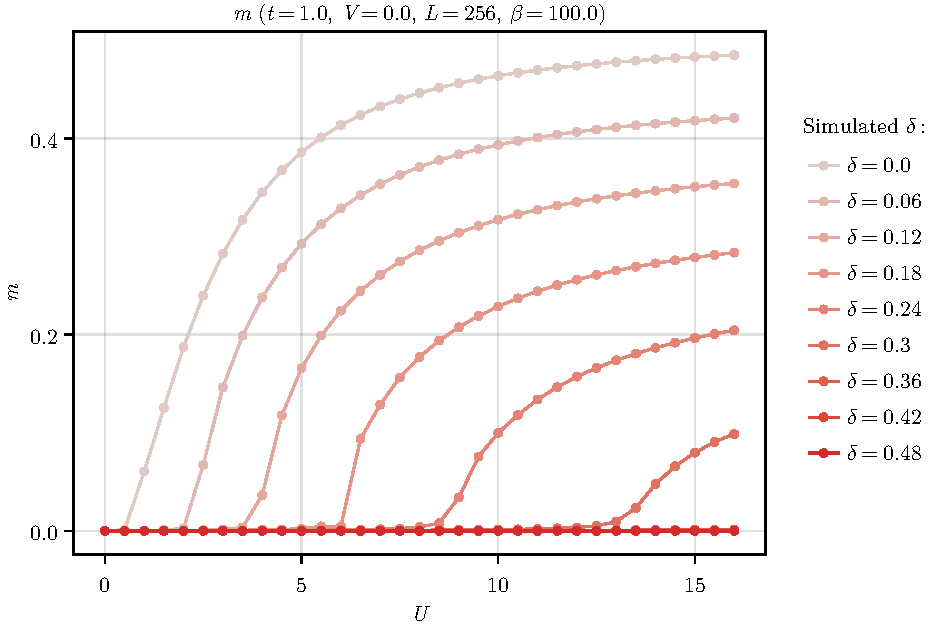
\includegraphics[height=0.32\linewidth]{../Project/plots/refined/Mode=hs/Phase=AF/Setup=D[256]/Syms=/RB=S/Obj=HFPs/xVar=U_pVar=δ/m_t=1.0_V=0.0_L=256_β=100.0.pdf}
		\label{appsubfig:mU-beta=100}
	}
	\subfloat[Doping $\delta = n-0.5$ dependence.]{
		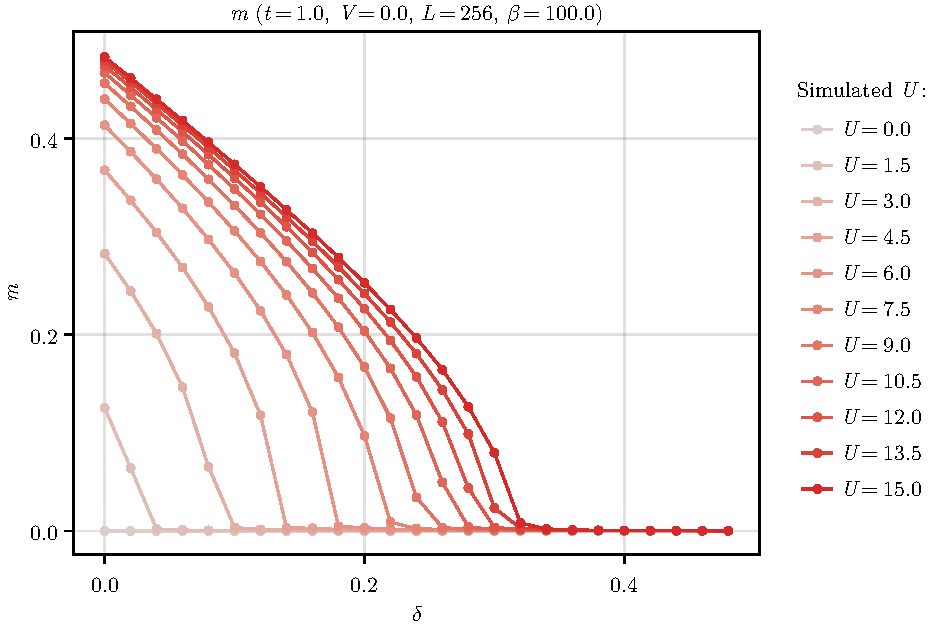
\includegraphics[height=0.32\linewidth]{../Project/plots/refined/Mode=hs/Phase=AF/Setup=D[256]/Syms=/RB=S/Obj=HFPs/xVar=δ_pVar=U/m_t=1.0_V=0.0_L=256_β=100.0.pdf}
		\label{appsubfig:dU-beta=100}
	}	
	\caption{Plots of the zero-temperature AF instability order parameter $m$ as a function of both the local repulsion $U/t$ (Fig.~\ref{appsubfig:mU-beta=100}) and the doping $\delta = n-1/2$ (Fig.~\ref{appsubfig:dU-beta=100}).}
	\label{appfig:mdU-beta=100}
\end{figure}


\section{Analytic expression of self-consistent magnetisation}

In this subsection we provide an analytic expression to compute $m$ self-consistently at half-filling. Multiply Eq.~\eqref{eq:af-hm-m-self-consistency} on both sides by $U$. Since due to symmetry $\mu=0$, we have the finite-temperature self-consistent equation
\[
\Delta = \frac{U}{L_xL_y} \sum_{\mathbf{k} \in \mathrm{MBZ}} \frac{\Delta}{\sqrt{\epsilon_{\mathbf{k}}^2 + \Delta^2}} \tanh(\frac{\beta}{2} \sqrt{\epsilon_{\mathbf{k}}^2 + \Delta^2})
\]
where we used the relation
\[
\mathrm{Th}_\mathbf{k}^{(-)}[\beta,0] = \tanh(\frac{\beta E_\mathbf{k}}{2})
\]
In thermodynamic limit $L \to \infty$
\[
\frac{1}{U} = \frac{1}{2} \int_\mathrm{BZ} \frac{\mathrm{d}\mathbf{k}}{(2\pi)^2} \frac{1}{\sqrt{\epsilon_{\mathbf{k}}^2 + \Delta^2}} \tanh(\frac{\beta}{2} \sqrt{\epsilon_{\mathbf{k}}^2 + \Delta^2})
\]
Substitute the momentum integral with an integral over energies:
\[
\frac{2}{U} = \int_{-4t}^{4t}  \frac{\mathrm{d}\epsilon \rho(\epsilon)}{\sqrt{\epsilon^2 + \Delta^2}} \tanh(\frac{\beta}{2} \sqrt{\epsilon^2 + \Delta^2})
\]
being $\rho(\epsilon)$ the $2$D square lattice DoS. Its explicit form is given by \cite{kogan2021greens}
\[
\rho(\epsilon) = \frac{1}{2\pi^2} K\left(
\sqrt{1 - \left(\frac{\epsilon}{4t} \right)^2}
\right)
\qquad
K(x) \equiv \int_0^{\pi/2} \frac{\mathrm{d}\theta}{\sqrt{1-x^2 \sin^2\theta}}
\]
$K(x)$ is the complete elliptic integral of the first kind, shown in Fig.~\ref{appsubfig:K(x)}.

\begin{figure}
	\centering
	\subfloat[Plot of $K(x)$.]{
		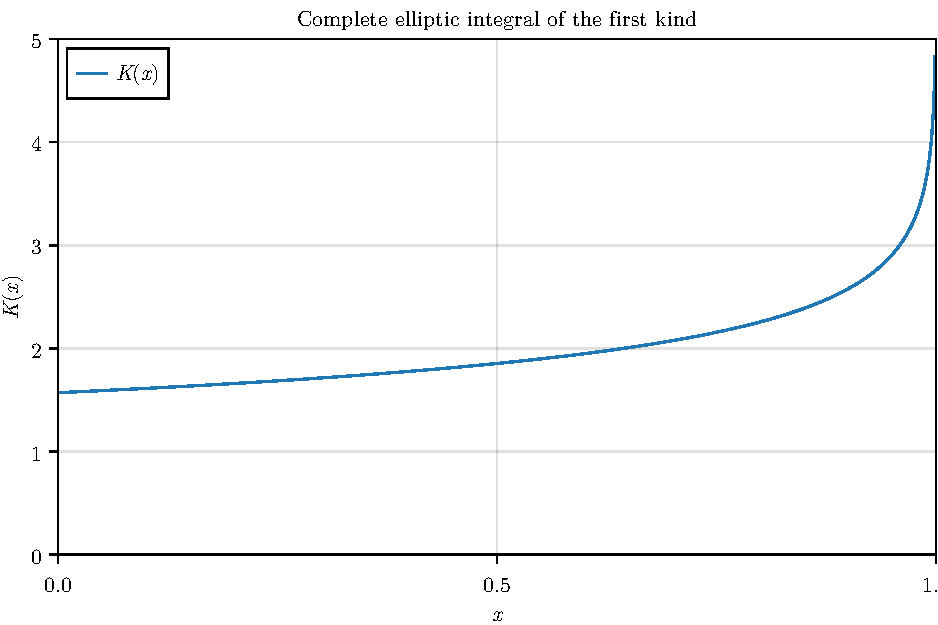
\includegraphics[height=0.32\linewidth]{../Project/src/labs/antiferromagnet-dos/K(x).pdf}
		\label{appsubfig:K(x)}
	}
	\subfloat[DoS and its approximation.]{
		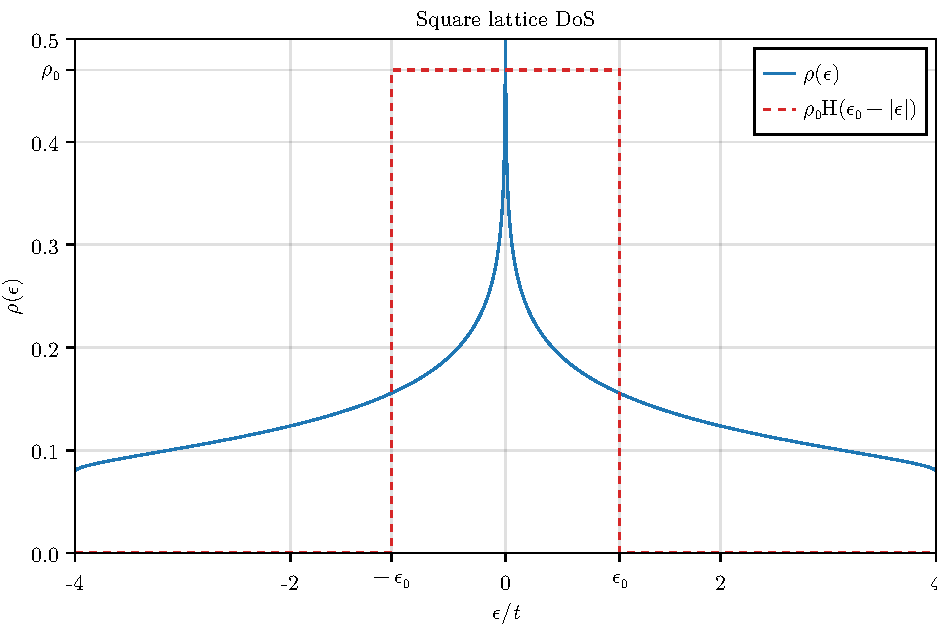
\includegraphics[height=0.32\linewidth]{../Project/src/labs/antiferromagnet-dos/D(x).pdf}
		\label{appsubfig:D(x)}
	}
	\caption{Plots of the complete elliptic integral of the first kind $K(x)$ and the density of states for the planar square lattice.}
	\label{appfig:square-dos}
\end{figure}

As is plotted in Fig.~\ref{appsubfig:D(x)}, the resulting DoS is logarithmically peaked at $\epsilon=0$, on the MBZ. An extremely rough but common approximation is to substitute the actual DoS with a step function,
\[
\rho(\epsilon) \simeq \rho_0 \mathrm{H} \left( \epsilon_0 - \abs{\epsilon} \right)
\qq{with}
2\rho_0\epsilon_0 = 1
\]
Here, the peak parameters $\epsilon_0$ and $\rho_0$ are chosen in order to maintain a correct DoS integral, considering also the $2$ pre-factor of spin degeneracy. Within this extremely rough approximation, we have
\[
\frac{2}{U} \simeq \rho_0 \int_{-\epsilon_0}^{\epsilon_0}  \frac{\mathrm{d}\epsilon}{\sqrt{\epsilon^2 + \Delta^2}} \tanh(\frac{\beta}{2} \sqrt{\epsilon^2 + \Delta^2})
\]
Suppose the system is magnetized, $\Delta>0$. At low temperature, $\beta \gg 1$, as a first approximation we can substitute the hyperbolic tangent with unity, obtaining
\[
\begin{aligned}
	\frac{2}{\rho_0 U} &\simeq \int_{-\epsilon_0}^{\epsilon_0}  \frac{\mathrm{d}\epsilon}{\sqrt{\epsilon^2 + \Delta^2}} \\
	&= \int_{-\epsilon_0/\Delta}^{\epsilon_0/\Delta}  \frac{\mathrm{d}x}{\sqrt{1+x^2}} \\
	&= \sinh^{-1} \left(\frac{\epsilon_0}{\Delta} \right) - \sinh^{-1} \left(-\frac{\epsilon_0}{\Delta} \right) \\
	&= 2\sinh^{-1} \left(\frac{\epsilon_0}{\Delta}\right)
\end{aligned}
\]
thus
\[
m \simeq \frac{\epsilon_0}{U\sinh(1/\rho_0 U)}
\]
having we used $\Delta = mU$. Now: at large $U$,
\[
\lim_{U\to +\infty} m \simeq \epsilon_0 \rho_0 = \frac{1}{2}
\]
which gives the correct saturation limit at high local repulsion. In the opposite limit,
\[
\begin{aligned}
	\lim_{U\to 0} m &\simeq \lim_{U\to 0} \frac{2\epsilon_0/U}{\exp(1/\rho_0 U)-\exp(-1/\rho_0 U)} \\
	&\simeq \lim_{U\to 0} \frac{2\epsilon_0}{U} \exp(-\frac{1}{\rho_0 U})
\end{aligned}
\]
giving a near-$0$ exponential suppression of magnetisation, typical of MFT self-consistent solutions.